
\documentclass[12pt,a4paper]{article}
\usepackage[latin1]{inputenc}
\usepackage{float}
\usepackage{amsmath}
\usepackage{amsfonts}
\usepackage{amssymb}
\usepackage{graphicx}
\usepackage{pdfpages}
\usepackage[hidelinks]{hyperref}

\begin{document}

	\begin{figure}
		\centering
		
\includegraphics[width=1.0\linewidth]{../assets/images/logo_poli.pdf}
	\end{figure}

\author{Giancarlo Danese - 945265\\
	Davide Savoldelli - 928676}
\date{A.Y. 2019/2020 - Prof. Di Nitto Elisabetta}


\title{
	\textbf{\Huge{SafeStreets}} \\
	\large Design Document
}



	\maketitle
	\newpage
	\tableofcontents
	\newpage

\section{INTRODUCTION}
\subsection{Purpose}
This document represents the Design Document (DD) for SafeStreets software and contains a functional description of the system. Since we provide an overall guide of the systems' architecture, it's addressed to the software development team
\subsection{Scope}
SafeStreets will have an embedded algorithm which will analyze pictures of the vehicle plates sent by the user in order to recognize the vehicle. This information, together with the position of the vehicle and the type of violation that has been committed, will be stored in the software's database.
\newline
Authorities will have the chance to mine the information retrieved in the database by highlighting the streets/areas in which most of the violations are committed, the type of vehicles which commit most of the violations and which type of violations occur the most, suggesting possible interventions that could be taken.	
\subsection{Definitions, Acronyms, Abbreviations}
			\begin{itemize}
				\item \texttt{User Device}: any compatible device with the SafeStreets application, like a smartphone or a computer
				\item \texttt{Personal Information}: information provided by the user during the registration process. It includes name, surname, birth date, address, e-mail address, mobile number.
				\item \texttt{Violation Report}: the act in which users can denounce violations on the streets, by providing the system its position, a photo and by selecting a violation from a precompiled menu
				\item \texttt{Mobile App}: an application that can be run by mobile devices, both smartphones and smartwatches.
				\item \texttt{Violations Map}: a map, accessible only by authorities, which contains notifications and alerts about all the unsafe areas where several violations are committed
			\end{itemize}
		\subsubsection{Acronyms}
			\begin{itemize}
				\item RASD: Requirements Analysis and Specification Document.
				\item DD: Design Document
				\item API: Application Programming Interface.
				\item GPS: Global Positioning System.
				\item PRA: Pubblico Registro Automobilistico
				\item AUC: Authority Unique Code
				\item DBP: Device-bound PIN
			\end{itemize}
\subsection{Revision History}
\subsection{Reference Documents}
\subsection{Document Structure}
\begin{itemize}
\item \textbf{1 Introduction} 
This section introduces the Design Document. It explains the Purpose, the Scope and the framework of the document.
\item \textbf{2 Architectural Design}
This section is focused on the main components used for this system and the relationship between them, providing information about their deployment and how they operate. It also focuses on the architectural
styles and the design patterns adopted for designing the system.
\item \textbf{3 User Interface Design}
This section provides an overview on how the User Interface will look like. In our case this section won't be detailed since all the product
functions have been already represented in the RASD.
\item \textbf{4 Requirements Traceability}
This section explains how the requirements defined in the RASD map to the design elements defined in this document.
\item \textbf{5 Implementation, Integration and Test Plan}
In this section we identify the order in which we plan to implement the subcomponents of the system and the order in which we plan to
integrate and test them.
\end{itemize}
\newpage
\section{ARCHITECTURAL DESIGN}
\subsection{High-level components and their interaction}
\begin{figure}[H]
		\centering
		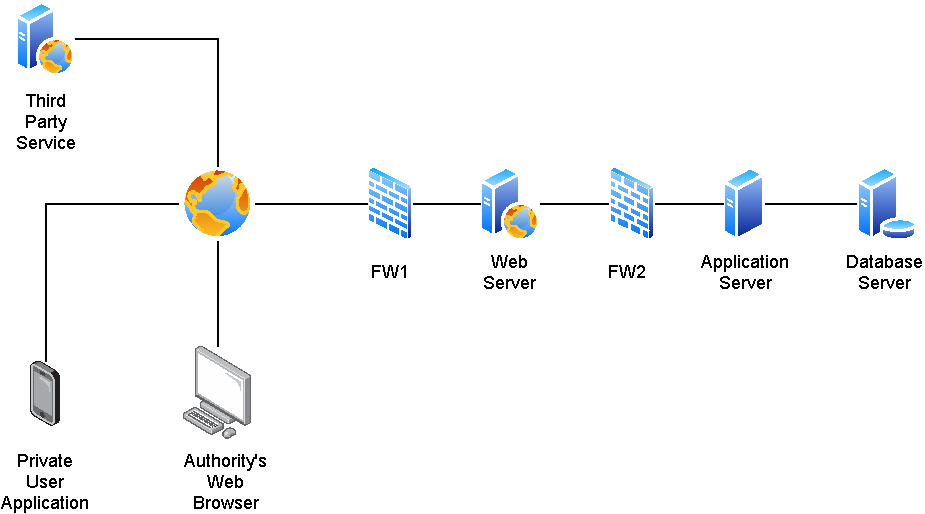
\includegraphics[width=0.9\linewidth]{../assets/sequence_diagrams/exports/architecture.pdf}
		\caption{High Level System Structure}
	\end{figure}
Our system can be summarized into 3 logical layers:
\begin{itemize}
\item \textbf{Presentation Layer}\\
This layer is divided into the Client tier (Mobile App for users) and the Web tier (Web App for authorities). From here, user, authorities and third parties, such as the municipality, can access the system's functionalities and the users' data through the Web Server, protected by a DeMilitarized Zone (DMZ)
\item \textbf{Application Layer}\\
In this layer the application server acts as a set of components accessible to the software developer through a standard API defined for the platform itself. We decided to separate the Application Server from the Web Server mainly for security reasons, and secondly because our application server targets much more than just Web page generation: it implements services like clustering and load-balancing.
\item \textbf{Data Layer}\\
Here we have the Database Server and the Database itself, where all the data about the users, the authorities and the violations reported are stored\\
\end{itemize}
\subsection{Component view}
\subsubsection{High Level Component Diagram}
The following diagrams represents the systems' components and its interfaces throughout which they interact in order to execute their functionalities. We'll divide this view into two sides, the Client side and the Server side:
\begin{itemize}
\item The Client side is composed of three different components, the \texttt{Authority Web Application}, intended for authorities only, the \texttt{Third Party Web Application}, for municipality, and the \texttt{Mobile Application}, for users. The first two refers to the \texttt{AuthoritiesWebServices} service for authorities and to the \texttt{Third Party Web Services} for the municipality, the last to the \texttt{UserMobileServices} service for users
\item The Server side is consequently also composed of three different components, the \texttt{Authorities Web Services} which will enable authorities to check the map, solve violations, etc., the \texttt{User Mobile Services} which gives users the chance to report street/parking violations with pictures, check/modify their personal data and review their report history.
\end{itemize}
\begin{figure}[H]
		\centering
		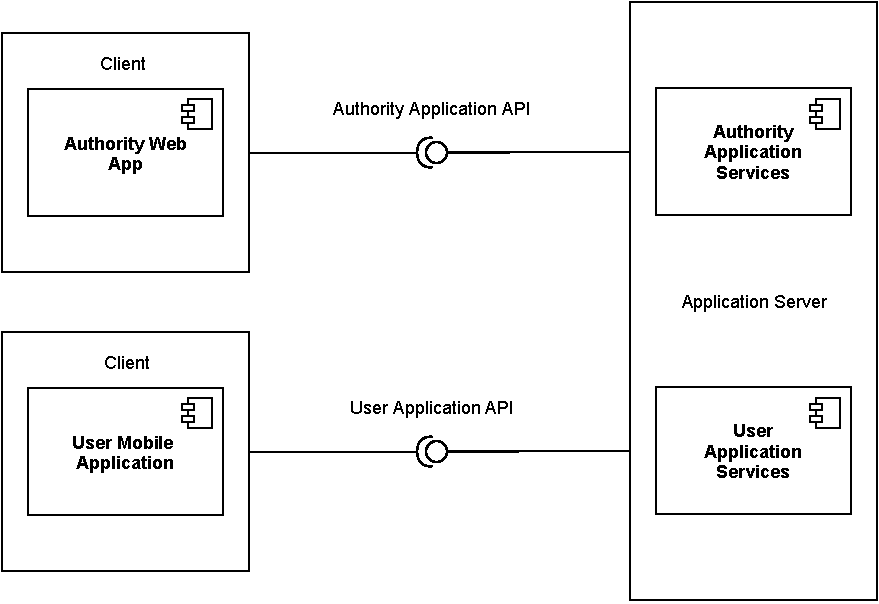
\includegraphics[width=1.2\linewidth]{../assets/images/component_no3rdparty.pdf}
	\end{figure}

\newpage
\subsubsection{User Mobile Application Projection}
The User Mobile Application Projection is subdivided into 4 modules: the \texttt{Authentication Module}, the \texttt{Profile Module}, the \texttt{Violations Report Module} and the \texttt{Main Thread Module}. These components need to communicate with the \texttt{User Service API} which exposes the application interfaces which will be described in the User Remote Services Projection. 
\begin{figure}[H]
		\centering
		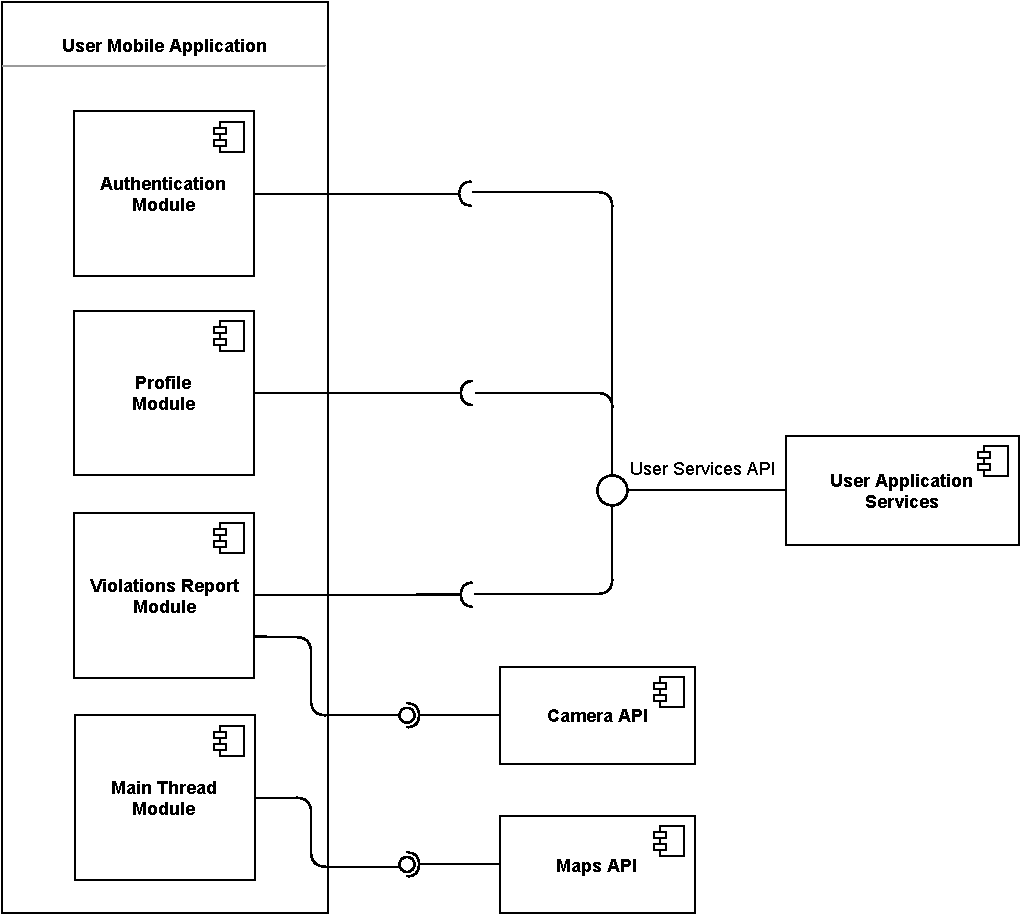
\includegraphics[width=1.2\linewidth]{../assets/images/user_mobile_projection.pdf}
	\end{figure}
As you can see, every single module but the Main Thread have access to the \texttt{User Application Services}. The \texttt{Violations Report Module}, the most important in the whole User Mobile Services, interfaces with a \texttt{Camera API}, enabled by the Oprative System (Android or iOS) and the external \texttt{Maps API}, provided by the Maps Provider.
\subsubsection*{Module Functionalities}
\begin{itemize}
\item \textbf{Authentication Module}: this module manages the registration and login processes of the user. It will allow them to insert their personal data and register to the system, and, subsequently, login with the same credentials. Eventually it provides the interface to manage and delete user profile.
\item \textbf{Violations Report Module}: this module is the most important as it enables the user to report street/parking violations by taking pictures of the vehicle involved and uploading them to the system. 
\item \textbf{Profile Module}: this module allows the mobile application to retrieve user's personal information, as well as the (private) history of submitted reports.
\item \textbf{Main Thread Module}: this module enables the default running of the Application. It is not directly connected to the remote API due to security concerns.\\\\
\end{itemize}
\subsubsection*{External Interface}
\begin{itemize}
\item \textbf{Camera API}: This is the API provided by default by the Operative System. It allows the Application to take pictures using the built-in camera.
\item \textbf{Maps API}: this is the API which allows the user to connect to a map service and download the maps basing on the actual location of the device. Since it is not the main concern of this document, for semplicity this "abstract" API represents both the GPS API provided by the OS and the remote Maps service.
\end{itemize}
\newpage
\subsubsection{User Remote Services Projection}
The User Services Projection is subdivided into 4 modules: the \texttt{Authentication Module}, the \texttt{Profile Module}, the \texttt{Violations Report Module} and the \texttt{OCR Module}. These components provide the User Mobile Application the following interfaces: \texttt{AuthenticationManager}, \texttt{ProfileManager} and \texttt{ViolationReportManager}. These components also need to communicate with a \texttt{DBMS} which must guarantee full availability and functionality to the Application for a correct user experience.
\begin{figure}[H]
		\centering
		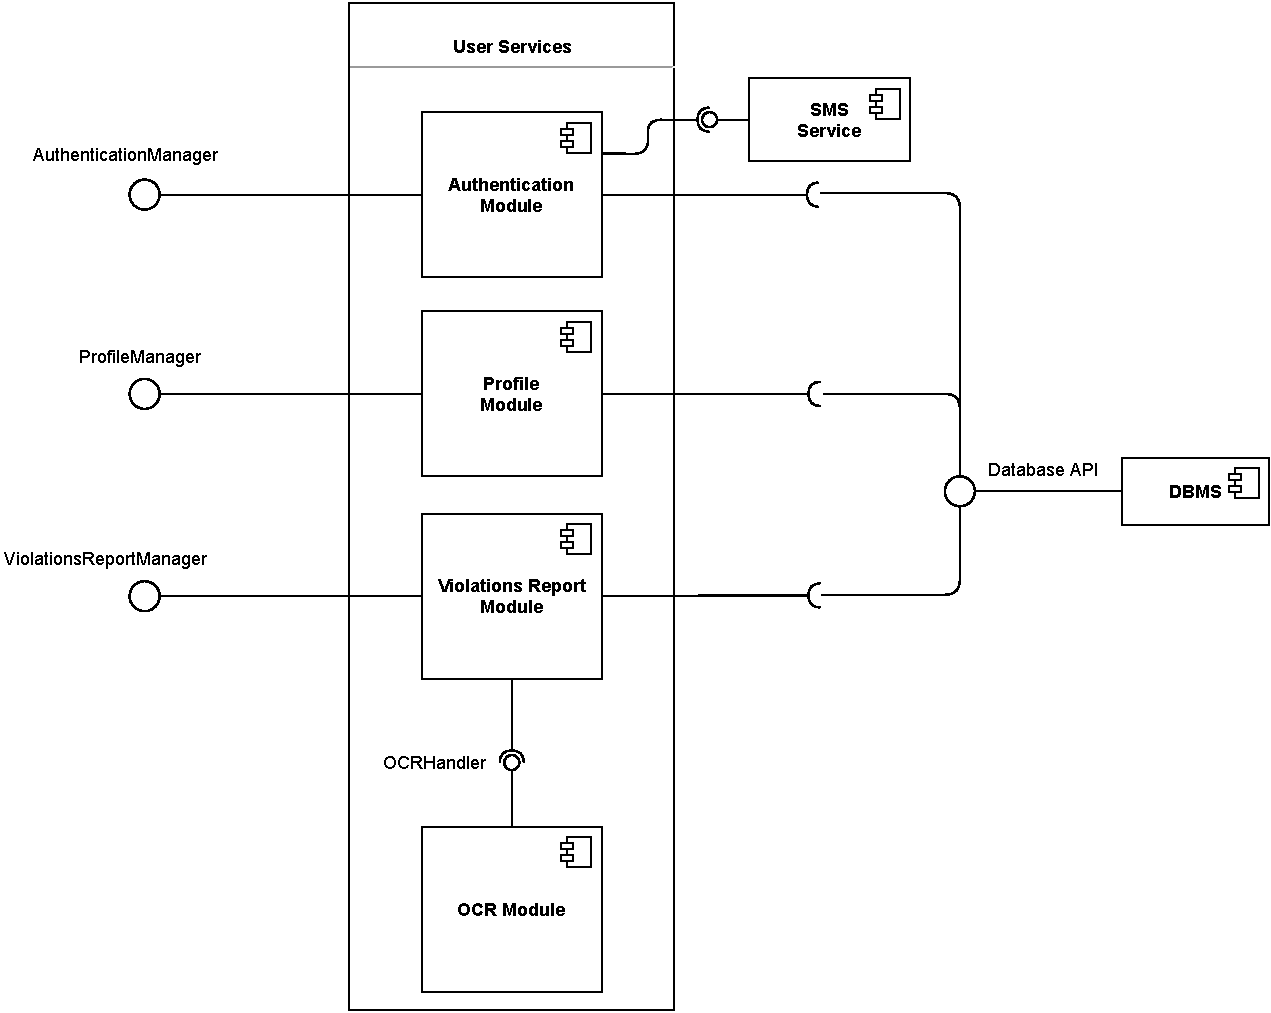
\includegraphics[width=1.2\linewidth]{../assets/images/user_projection.pdf}
	\end{figure}
Every single module but the \texttt{OCR Module} have access to the \texttt{DBMS} and the \texttt{Authentication Module} interacts with a \texttt{SMS Service}, where a SMS is sent with a verification code to subscribe to the system. The \texttt{Violations Report Module}, the most important in the whole User Mobile Services, interfaces with a \texttt{OCRHandler} which tries to recognize the license plate from the photo and saves it in the Violation Report.
\subsubsection*{Module Functionalities}
\begin{itemize}
\item \textbf{Authentication Module}: this module manages the registration and login processes of the user in the remote application. It accepts incoming personal data from the Mobile App and guarantees the correct login/registration process, retrieving data from the Database.
\item \textbf{Violations Report Module}: this core module receives the violations made from the Mobile App, validates them and eventually add or update them to Database.
\item \textbf{Profile Module}: this modules receives all the requests coming from the Mobile Application concerning the retreival of the  user's personal information. It asks the Database and forwards responses to the user. The information provided includes personal data of the user and his/her reports history.
\item \textbf{OCR Module}: this module provides all the necessary functions concerning the automatic detection of the plate number based on image recognition algorithms.\\\\
\end{itemize}
\subsubsection*{External Interface}
\begin{itemize}
\item \textbf{SMS Service}: this module manages the SMS sending to the user mobile application in order to complete the registration process and/or reset password in case of loss.
\end{itemize}
\newpage
\subsubsection{Authority Web Application Projection}
The Authority Web Services Projection is subdivided into 4 modules: the \texttt{Authentication Module}, the \texttt{Profile Module}, the \texttt{Violation Retrieve Module} and the \texttt{Suggestion Module}. These components also need to communicate with a \texttt{Authority Service API} which exposes the application interfaces which will be described in the Authority Remote Services Projection.
\begin{figure}[H]
		\centering
		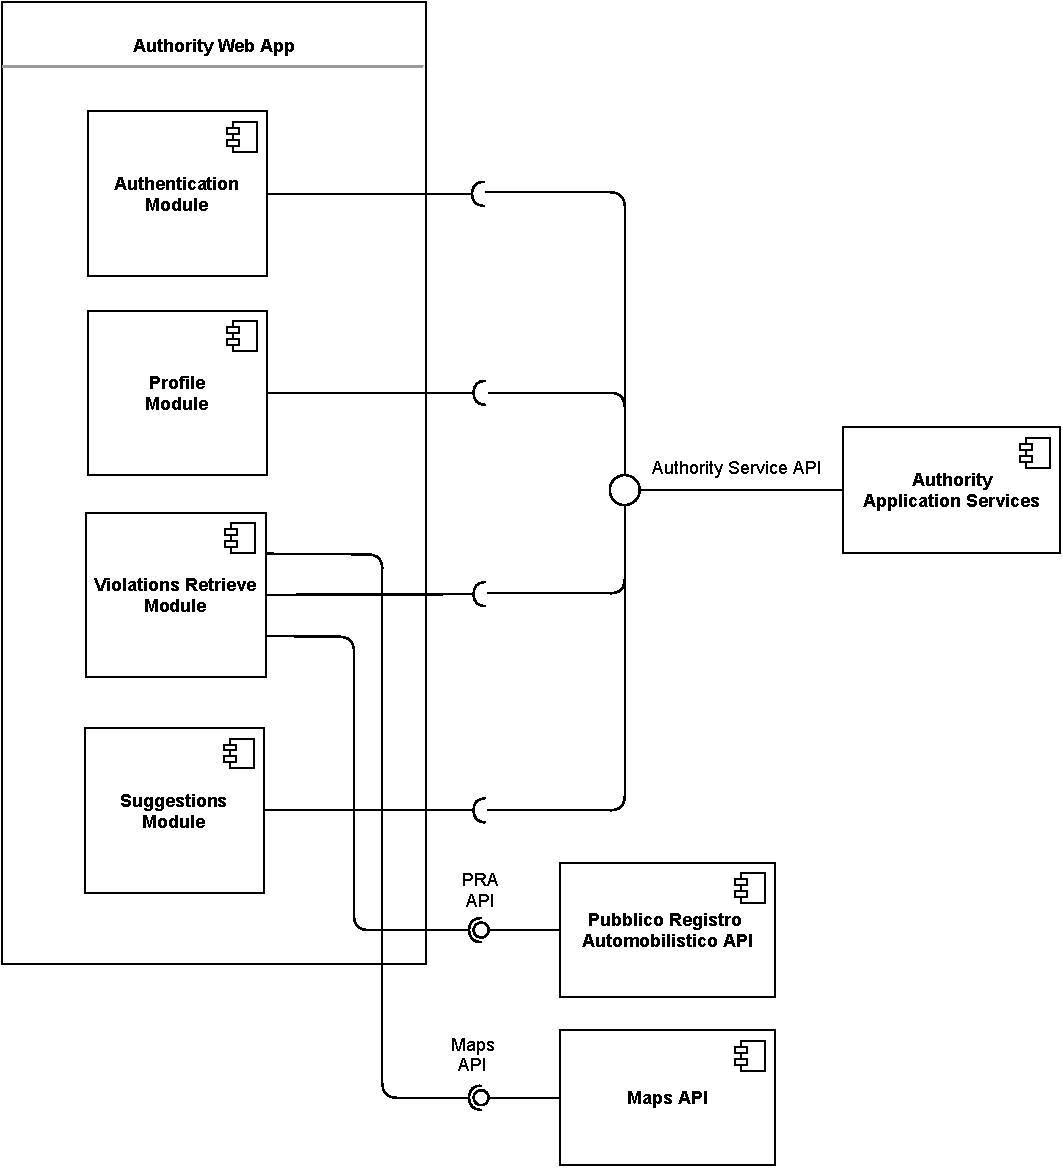
\includegraphics[width=1.1\linewidth]{../assets/images/Authority_webapp_projection.pdf}
	\end{figure}
\newpage
\subsubsection*{Module Functionalities}
\begin{itemize}
\item \textbf{Authentication Module}: this module manages the registration and login of the authority. It will allow them to insert their personal data and to receive their AUC and DBP in order to successfully register to the system.
\item \textbf{Profile Module}: this module deals with the access to the personal information of the Authority.
\item \textbf{Violation Retrieve Module}: this module lets the authority interact with the list of violations, checking their validity and solving them. 
\item \textbf{Suggestion Module}: this module manages the dispatching of suggestions to the Authority about possible interventions to take in order to prevent violations from being committed in that precise area.
\end{itemize}
\subsubsection*{External Interface}
\begin{itemize}
\item \textbf{Pubblico Registro Automobilistico API}: this module allows the Authority to retrieve all the available public information of a driver (Name, Surname, Car Model, Insurance data) basing on a valid registered plate number.
\item \textbf{Maps API}: this module downloads the actual maps for the Web Application basing on the virtual position of the cursor.
\end{itemize}
\newpage
\subsubsection{Authority Remote Services Projection}
The Authority Web Services Projection is subdivided into 5 modules: the \texttt{Authentication Module}, the \texttt{Profile Module}, the \texttt{Violation Retrieve Module}, the \texttt{Suggestion Module} and the \texttt{Machine Learning Module}. These components provide to the Authority Web Application the following interfaces: \texttt{AuthenticationManager}, \texttt{ProfileManager}, \texttt{ViolationRetriveManager} and \texttt{SuggestionManager} . These components also need to communicate with a \texttt{DBMS} for the correct dispatching of data.
\begin{figure}[H]
		\centering
		\includegraphics[width=1.2\linewidth]{../assets/images/authority_projection.pdf}
	\end{figure}
We can see here how the \texttt{Suggestion Module} refers to the \texttt{Machine Learning Module} in order to generate suggestions for interventions to take in streets particularly full of violations.
\subsubsection*{Module Functionalities}
\begin{itemize}
\item \textbf{Authentication Module}: this module manages the registration and login of the authority. It will validate Authority AUC and DBP in order to provide the Authority a secured login.
\item \textbf{Profile Module}: this module accepts Authority's requests about personal information, gets them from the Database and forwards them to the Web App.
\item \textbf{Violation Retrieve Module}: this dispatch the Violation Information to the Authority's Web App.
\item \textbf{Suggestion Module}: this module manages the dispatching of suggestions to the Authority's Web App. It also retrieves Violations' data from the enterprise database and the Accidents' data provided by the municipality's external API. This data is finally sent through the \texttt{MachineLearningHandler} interface in order to provide its actual computation.
\item \textbf{Machine Learning Module}: this module allows the generation of suggestions basing on the data (Violations and Accidents) exchanged with the suggestion module.
\end{itemize}
\subsubsection*{External Interface}
\begin{itemize}
\item \textbf{Municipality's Accidents Service}: this module allows the retrieval of the data about the accidents related to the area of interest in order to complete the Suggestions' computation.
\end{itemize}
\subsection{Component interfaces}
\begin{figure}[H]
		\centering
		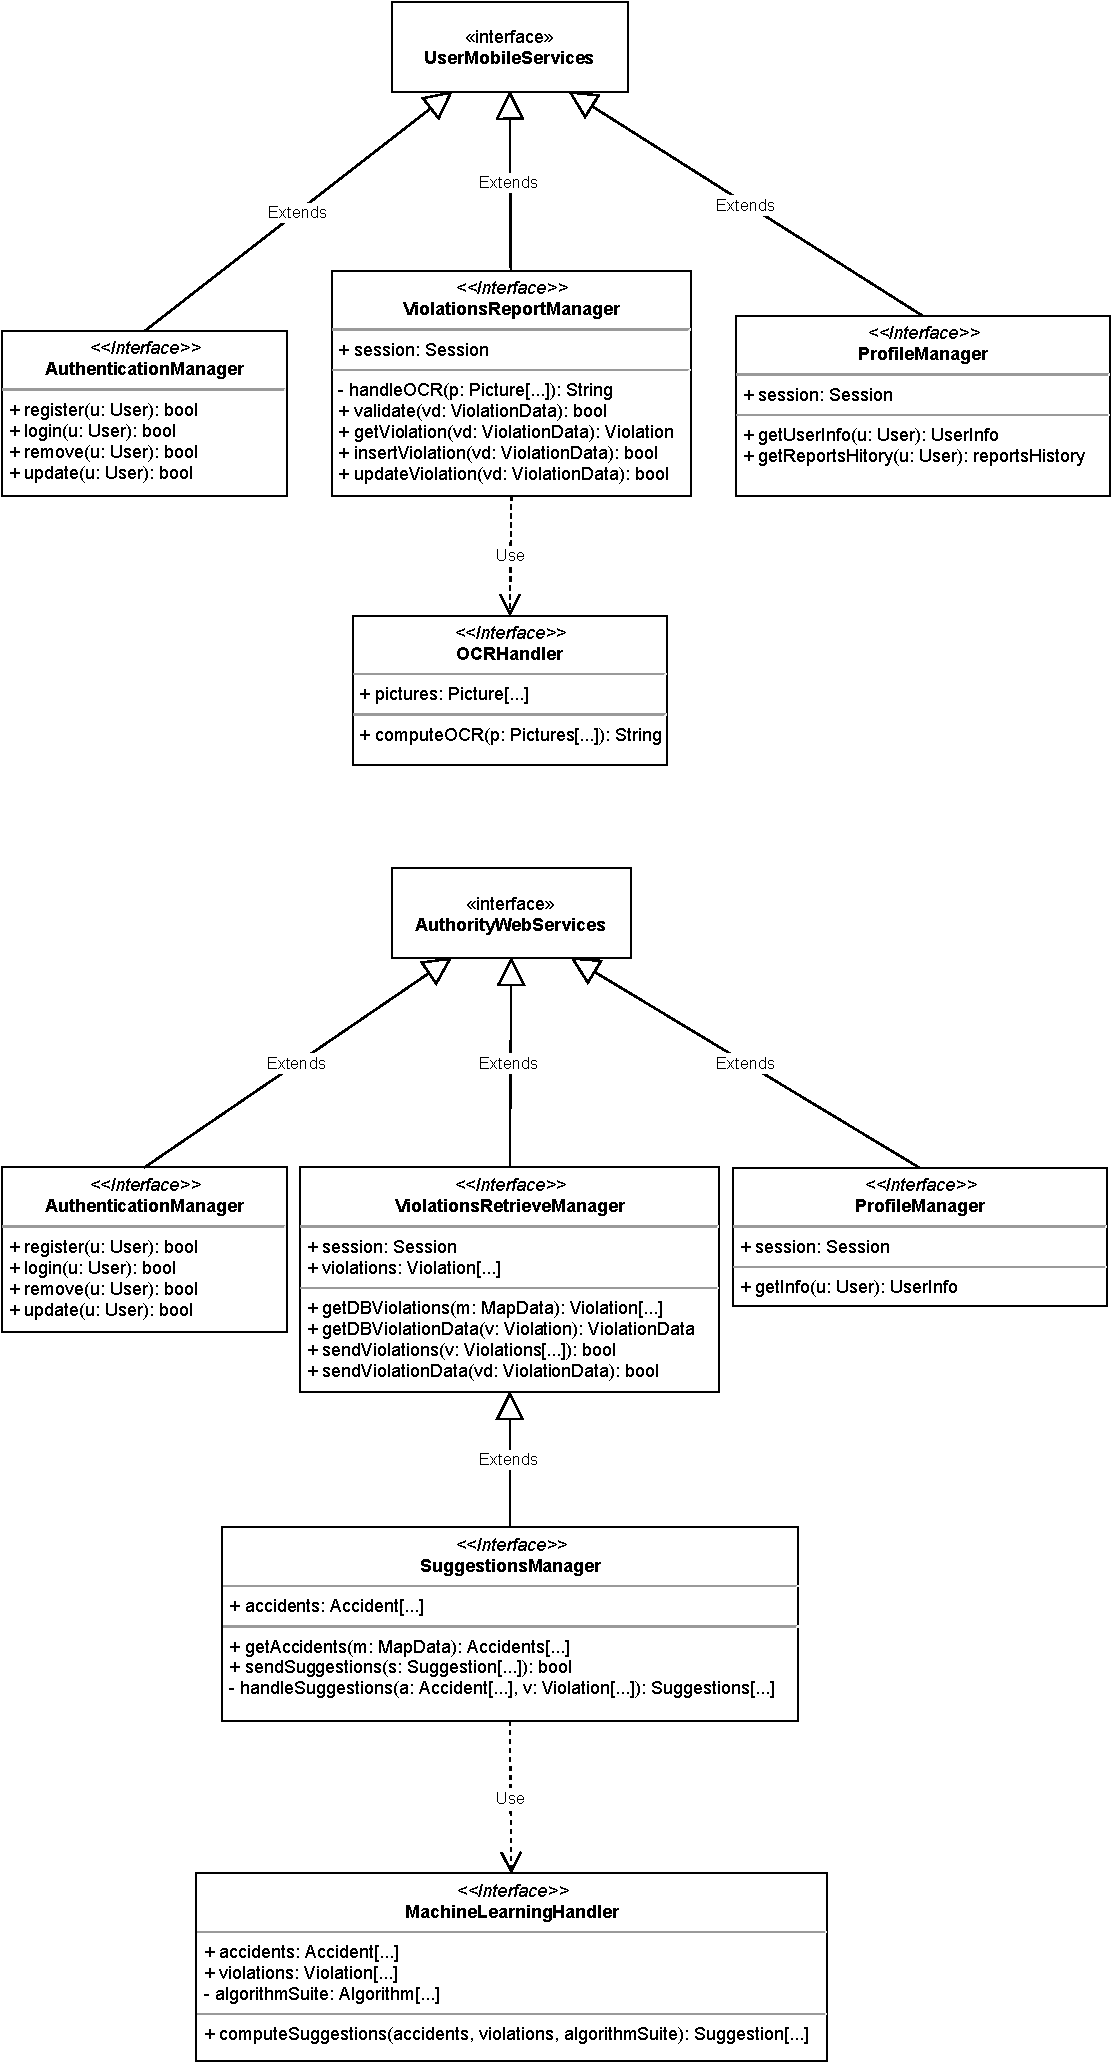
\includegraphics[width=0.7\linewidth]{../assets/images/component_interfaces1.pdf}
	\end{figure}
\subsubsection{External Interfaces}
SafeStreets uses some Application Programming Interfaces to facilitate the implementation. These components are infact largely used and compatible with most of the devices currently on the market:
\begin{itemize}
\item \texttt{SMS API}: it enables the the possibility to register to the system with a telephone number, thanks to a process in which a temporary code is sent through an SMS Service
\item \texttt{Maps API}: fundamental for the violation reporting functionality, as it shows the user its location and the vehicles location in a well visible map. It is also used by the Authority Web App to display the Violations and the Suggestions in the selected area.
\item \texttt{Camera API}: every users' smartphone needs direct access to its camera to take pictures of the violation-committing vehicles' license plate.
\item \texttt{PRA API}: the Pubblico Registro Automobilistico is the big database where any user can infer sensible data regarding a vehicles' owner. In our case, the PRA is accessed by authorities in the process we called Violation Solving where they can take measures towards the vehicles owner
\item \texttt{Accidents API}: this API allows the Suggestions Module to retreive data about the accidents happened in a specific area. Combining this data with the violations reported by users, the Authority is provided accurate suggestions in order to prevent future violations.
\item \texttt{Database API}: this API is actually used to support multiple database servers easily, to provide a structured interface for the dynamic construction of queries, to enforce security checks and to facilitate the interaction with the database
\end{itemize}
\newpage
\subsection{Deployment view}
In order to deploy the system, we decided to implement a 4-tier architecture:
\begin{itemize}
\item \textbf{Tier 1}
The first tier will be composed by the Client (we opted for a Thin Client) that includes a Mobile Application (for users) and a Web Application (for authorities).\\\\
\begin{figure}[H]
		\centering
		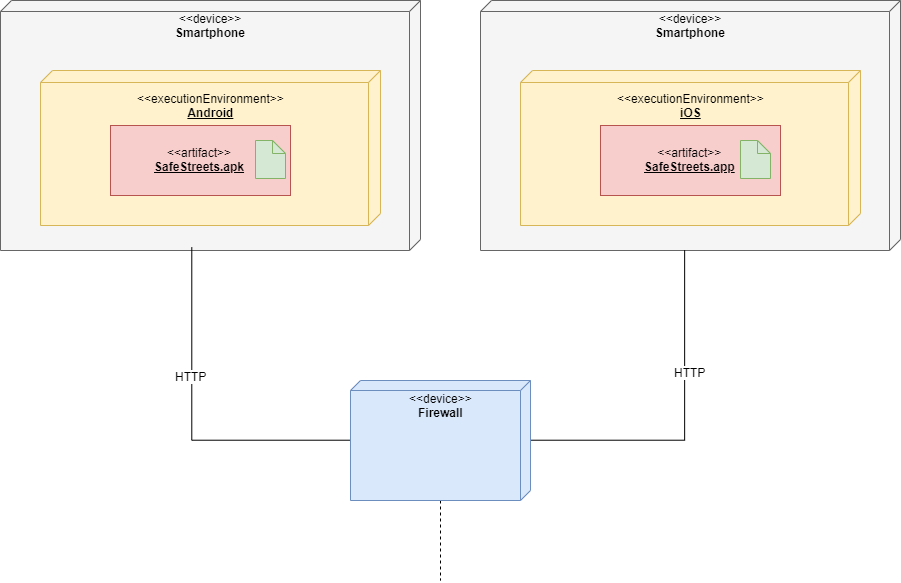
\includegraphics[width=1.0\linewidth]{../assets/images/MOBILE APPLICATION COMP VIEW.png}
		\caption{Tier 1 Deployment View}
	\end{figure}
\newpage
\item \textbf{Tier 2}
This tier corresponds to the Web Server, whose main focus is to store, process static content and deliver web pages to the Clients. Infact, we opted for Apache Tomcat thanks to its high-availability, clustering feature for load balancing and its optimal java-focused environment\\\\
\begin{figure}[H]
		\centering
		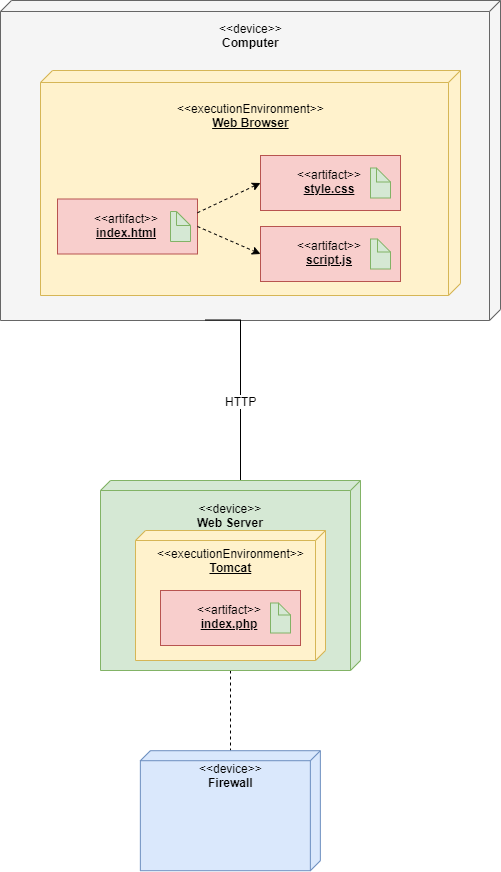
\includegraphics[width=0.5\linewidth]{../assets/images/tier1_tier2.png}
		\caption{Tier 2 Deployment View}
	\end{figure}
\newpage
\item \textbf{Tier 3}
This tier corresponds to the Application Server, that both facilitates the creation of web applications and provides a server environment where to run these applications. We opted for Apache Geronimo, since one of its components is Tomcat, and because of its compatibility with Java EE 6 specifications.\\\\
\begin{figure}[H]
		\centering
		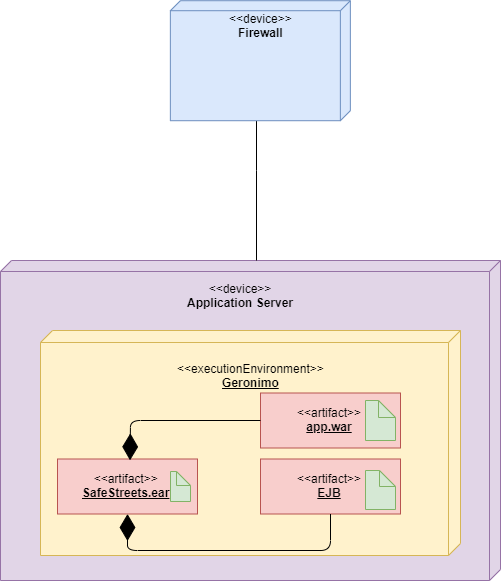
\includegraphics[width=0.5\linewidth]{../assets/images/app_server.png}
		\caption{Tier 3 Deployment View}
	\end{figure}
\newpage
\item \textbf{Tier 4}
The final tier corresponds to the Database Server, where the DBMS is running. We opted for MySQL, since it is one of the most secure and reliable database management system used in popular web applications, while at the same time guarantees scalability and high performance.
\begin{figure}[H]
		\centering
		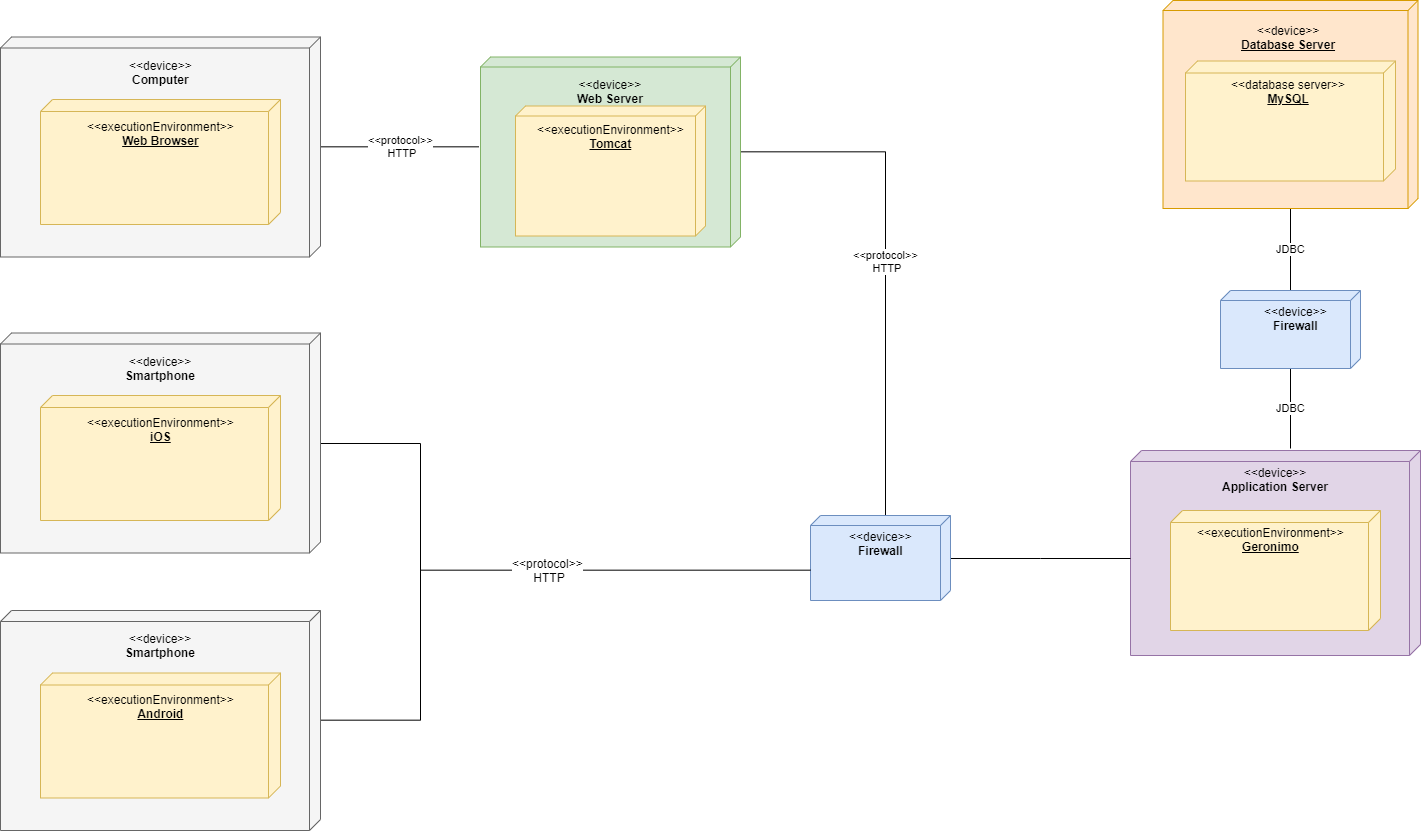
\includegraphics[width=1.0\linewidth]{../assets/images/ENTIRE SYSTEM.png}
		\caption{Entire System Deployment View with Tier 4}
	\end{figure}
\end{itemize}
\subsection{Runtime view}
\subsubsection{Violation Report}
\begin{figure}[H]
		\centering
		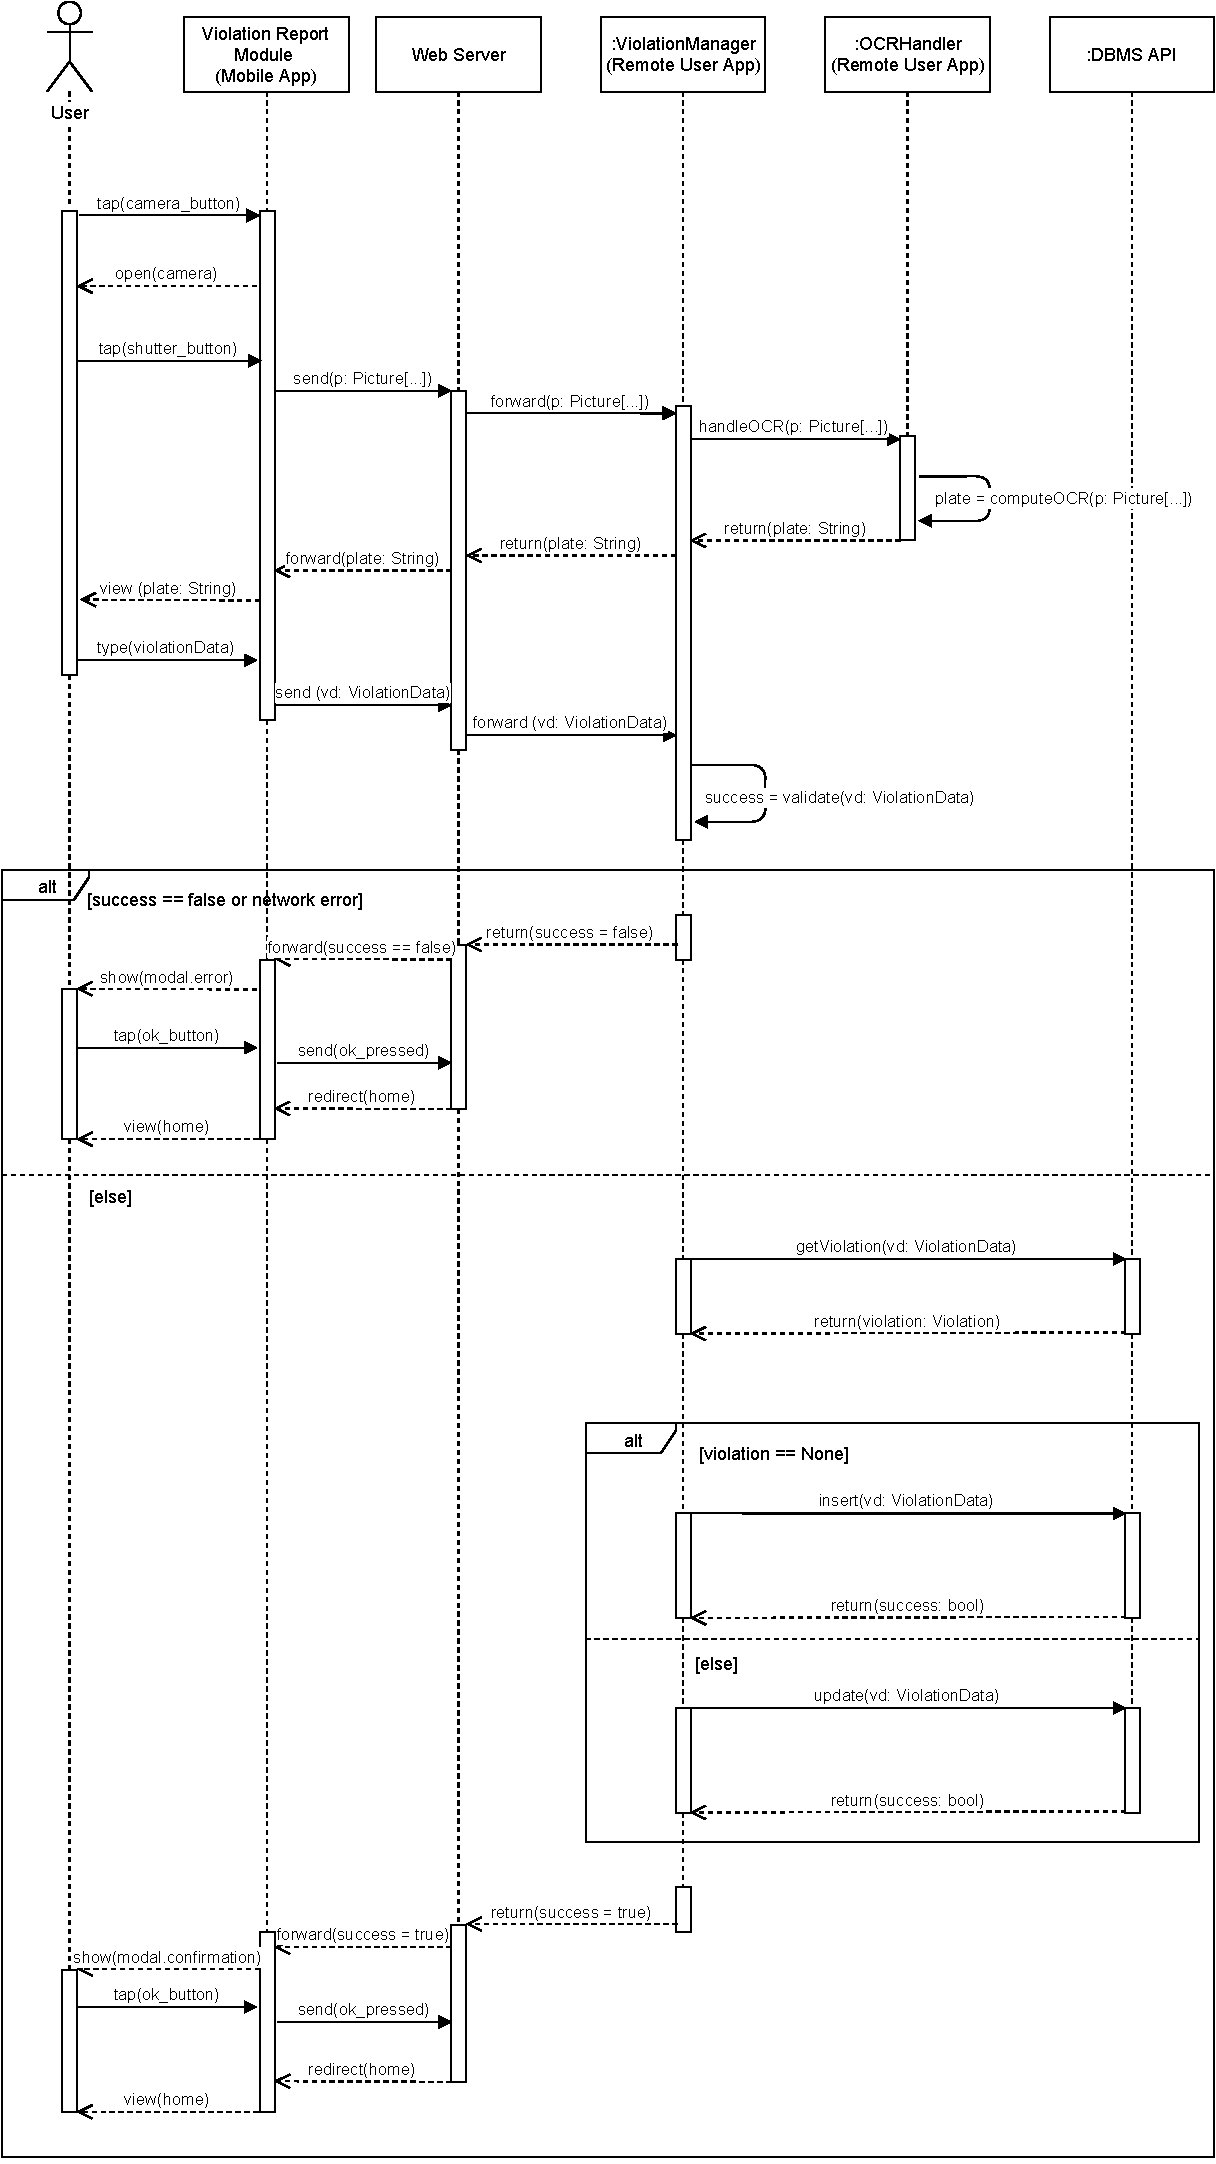
\includegraphics[width=0.7\linewidth]{../assets/sequence_diagrams/exports/workflw_violation_report_complete.pdf}
		\caption{Workflow of Violation Reporting.}
	\end{figure}
In this sequence diagram the process of violation reporting is shown. The process starts with the user's click on camera button, the requests are sent to a Web Server which forwards them to the ViolationManager interface of the Application Server. It calls first the OCRHandler to recognize the plate number and then sends it to the user. The user is now allowed to complete the Violation data (such as uploading pictures, giving a description and choosing the category of violation). After the Violation Data is validated by the Violation Module, in case of success, the item is first queried from the Database and inserted or updated into it. In case of failure an error message is show to the user.
\newpage
\subsubsection{Violation Retrieval}
\begin{figure}[H]
		\centering
		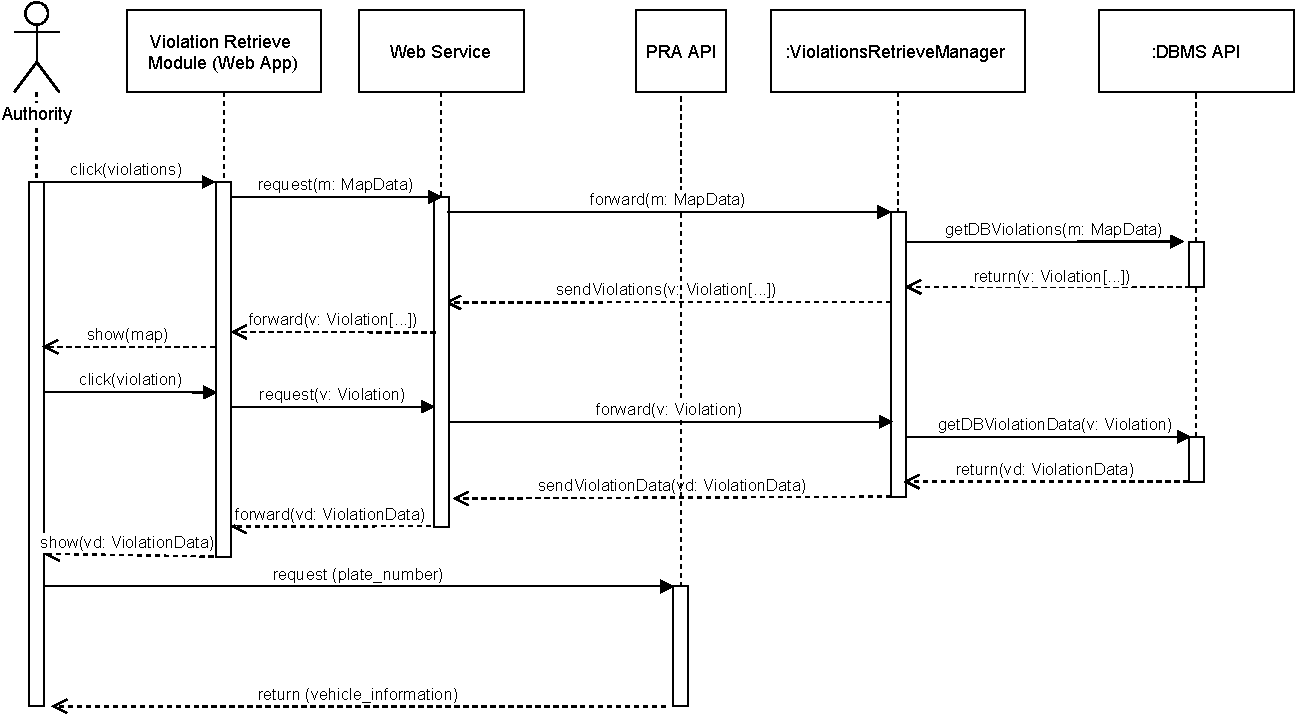
\includegraphics[width=1.0\linewidth]{../assets/sequence_diagrams/exports/workflw_violation_retrieval_complete.pdf}
		\caption{Workflow of Violation Retrieval.}
	\end{figure}
In this sequence diagram the process of Violation retrieval is shown. The authority selectes the displaying of the Violations in the Web Application, basing on the selected map location. The request is sent to the ViolationRetrieveManager interface of the Authority Module in the Application Server. The request is sent to the Database and finally forwarded to the Authority. When the Authority clicks on a Violation a new requenst is generated: the ViolationRetrieveManager ask the Database again to access the data of a specific violation. The data is sent back to the Authority passing through the Web Server.
\subsubsection{Suggestion Retrieval}
\begin{figure}[H]
		\centering
		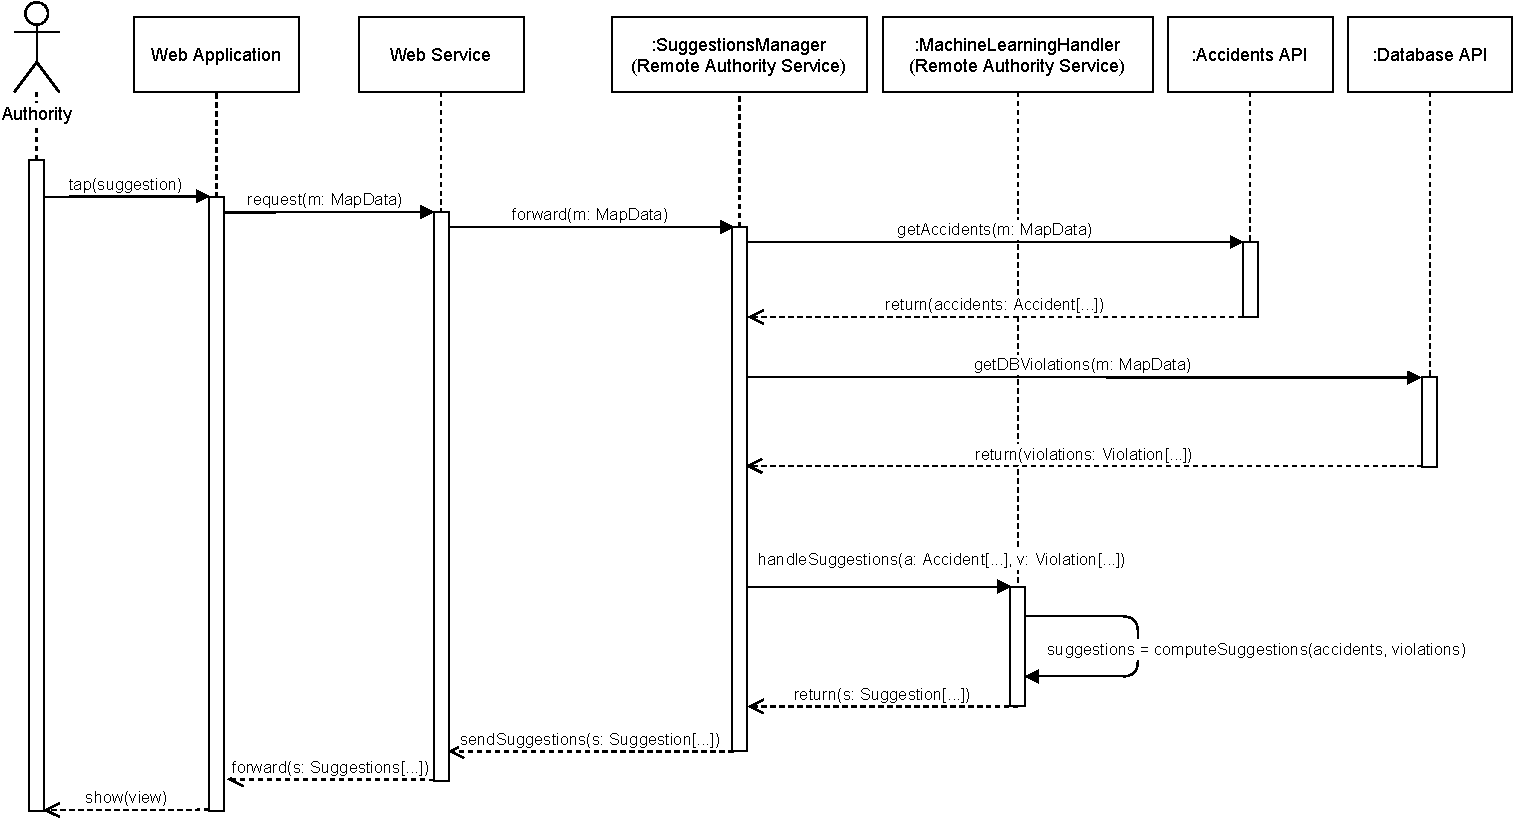
\includegraphics[width=1.0\linewidth]{../assets/sequence_diagrams/exports/workflw_suggestions_complete.pdf}
		\caption{Workflow of Suggestion computation and displaying.}
	\end{figure}
In this sequence diagram the process of Suggestion retrieval is shown. The Authority asks for the displaying of the suggestion related to a specific map location. The request is sent to the SuggestionManager interface, which first asks the external Accidents API provided by the municipality to retrieve the Accidents in the area. Then a new request for the violations to the DBMS API is sent and when the Suggestion Module has got the whole data, it calls the MachineLearningHandler to compute new Suggestions, basing on the actual data. The response is then sent back to the Authority passing through the Web Server.
\newpage
\subsection{Selected architectural styles and patterns}
\subsubsection{Design Patterns}
Here are the design patterns we used to make our architecture more flexible:
\begin{itemize}
\item \textbf{Model View Controller}\\
Nowadays, most Mobile and Web Applications rely on this pattern. These type of applications infact retrieve data from the Database and updates the Users' Interface consequently and according to the provided input, while the Controller checks the validity of the requested operations. Therefore the main scope of this pattern is to separate the Data (Model), the Users' Interface (View) and the user's input validator (Controller)
\begin{figure}[H]
		\centering
		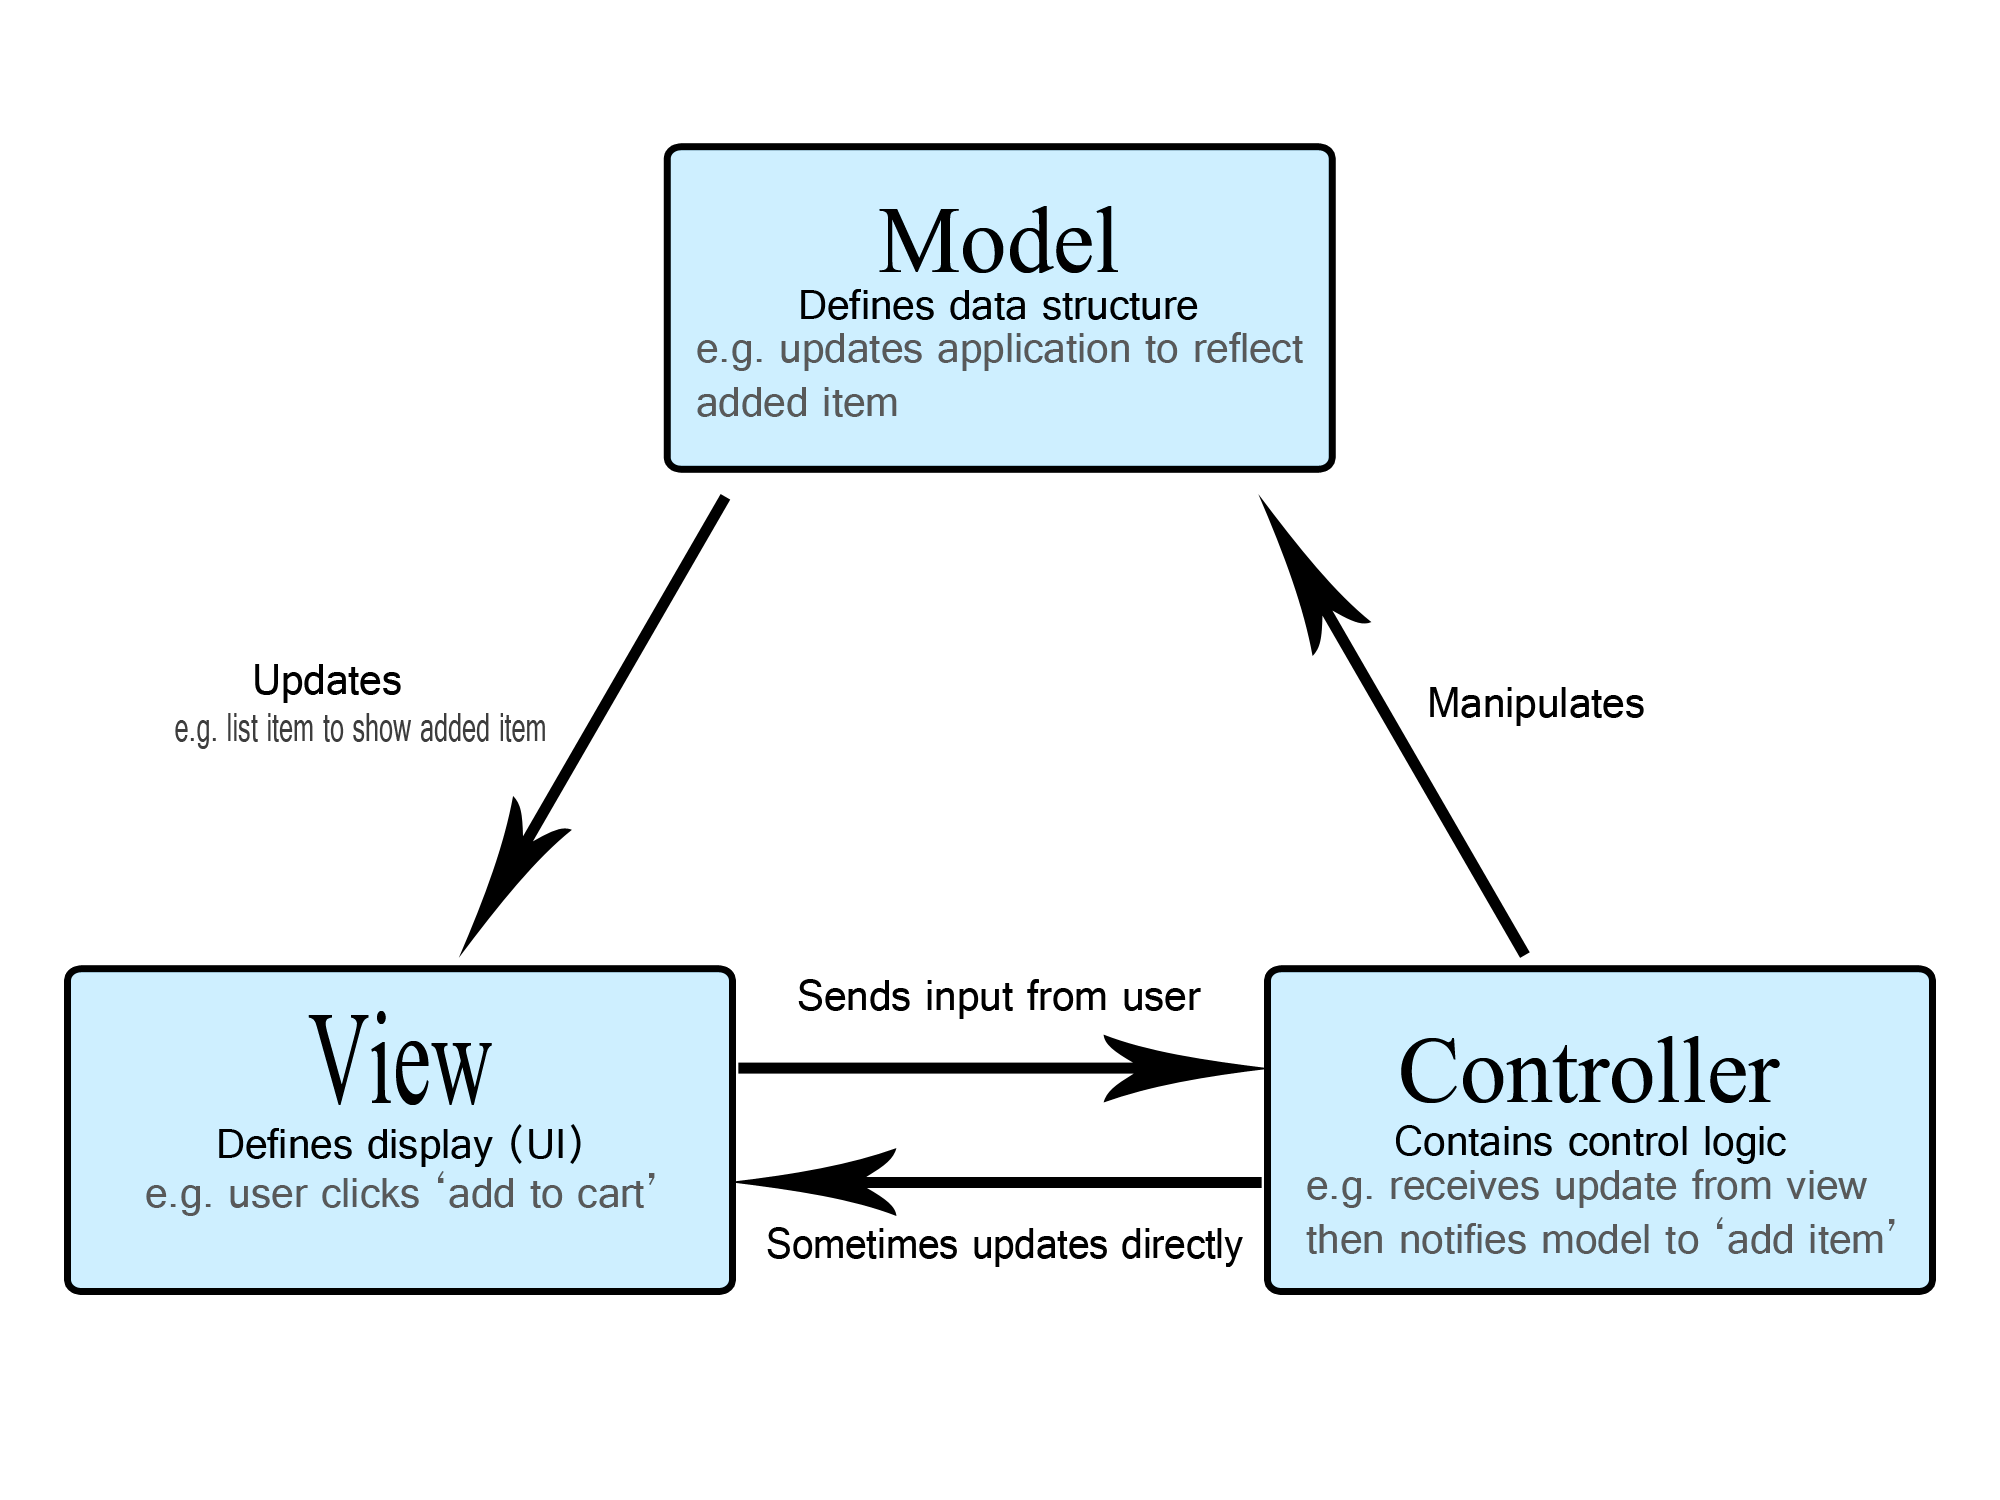
\includegraphics[width=1.0\linewidth]{../assets/images/model-view-controller-light-blue.png}
	\end{figure}
\newpage
\item \textbf{Decorator Pattern}\\
The Decorator is a design pattern that allows behavior to be added to an individual object, dynamically, without affecting the behavior of other objects from the same class. It can be used to extend (decorate) the functionality of a certain object statically, or in some cases at run-time, independently of other instances of the same class, provided some groundwork is done at design time. This is achieved by designing a new Decorator class that wraps the original class. This pattern is designed so that multiple decorators can be stacked on top of each other, each time adding a new functionality to the overridden method. In our case, it can be used to add new information on a already reported violation which lacks in important data without affecting the other violations already compiled
\begin{figure}[H]
		\centering
		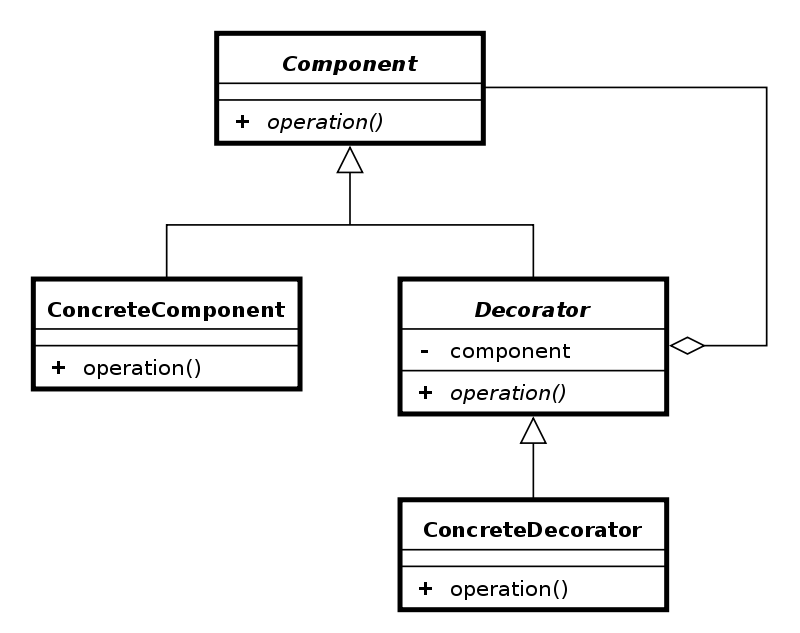
\includegraphics[width=1.0\linewidth]{../assets/images/800px-Decorator_UML_class_diagram.png}
	\end{figure}
\newpage
\item \textbf{Proxy Pattern}\\
It provides a surrogate for another object to control access to it. In our system architecture it can be useful to interface the Application Server with the Database Server. For example, whenever a user, an authority or a third party (municipality) requests some data that is unchanged, the proxy can answer the query without involving access to the database, providing a better response time. In our case, it can be useful when a user requests his reports history or when an authority requests a suggestion
\begin{figure}[H]
		\centering
		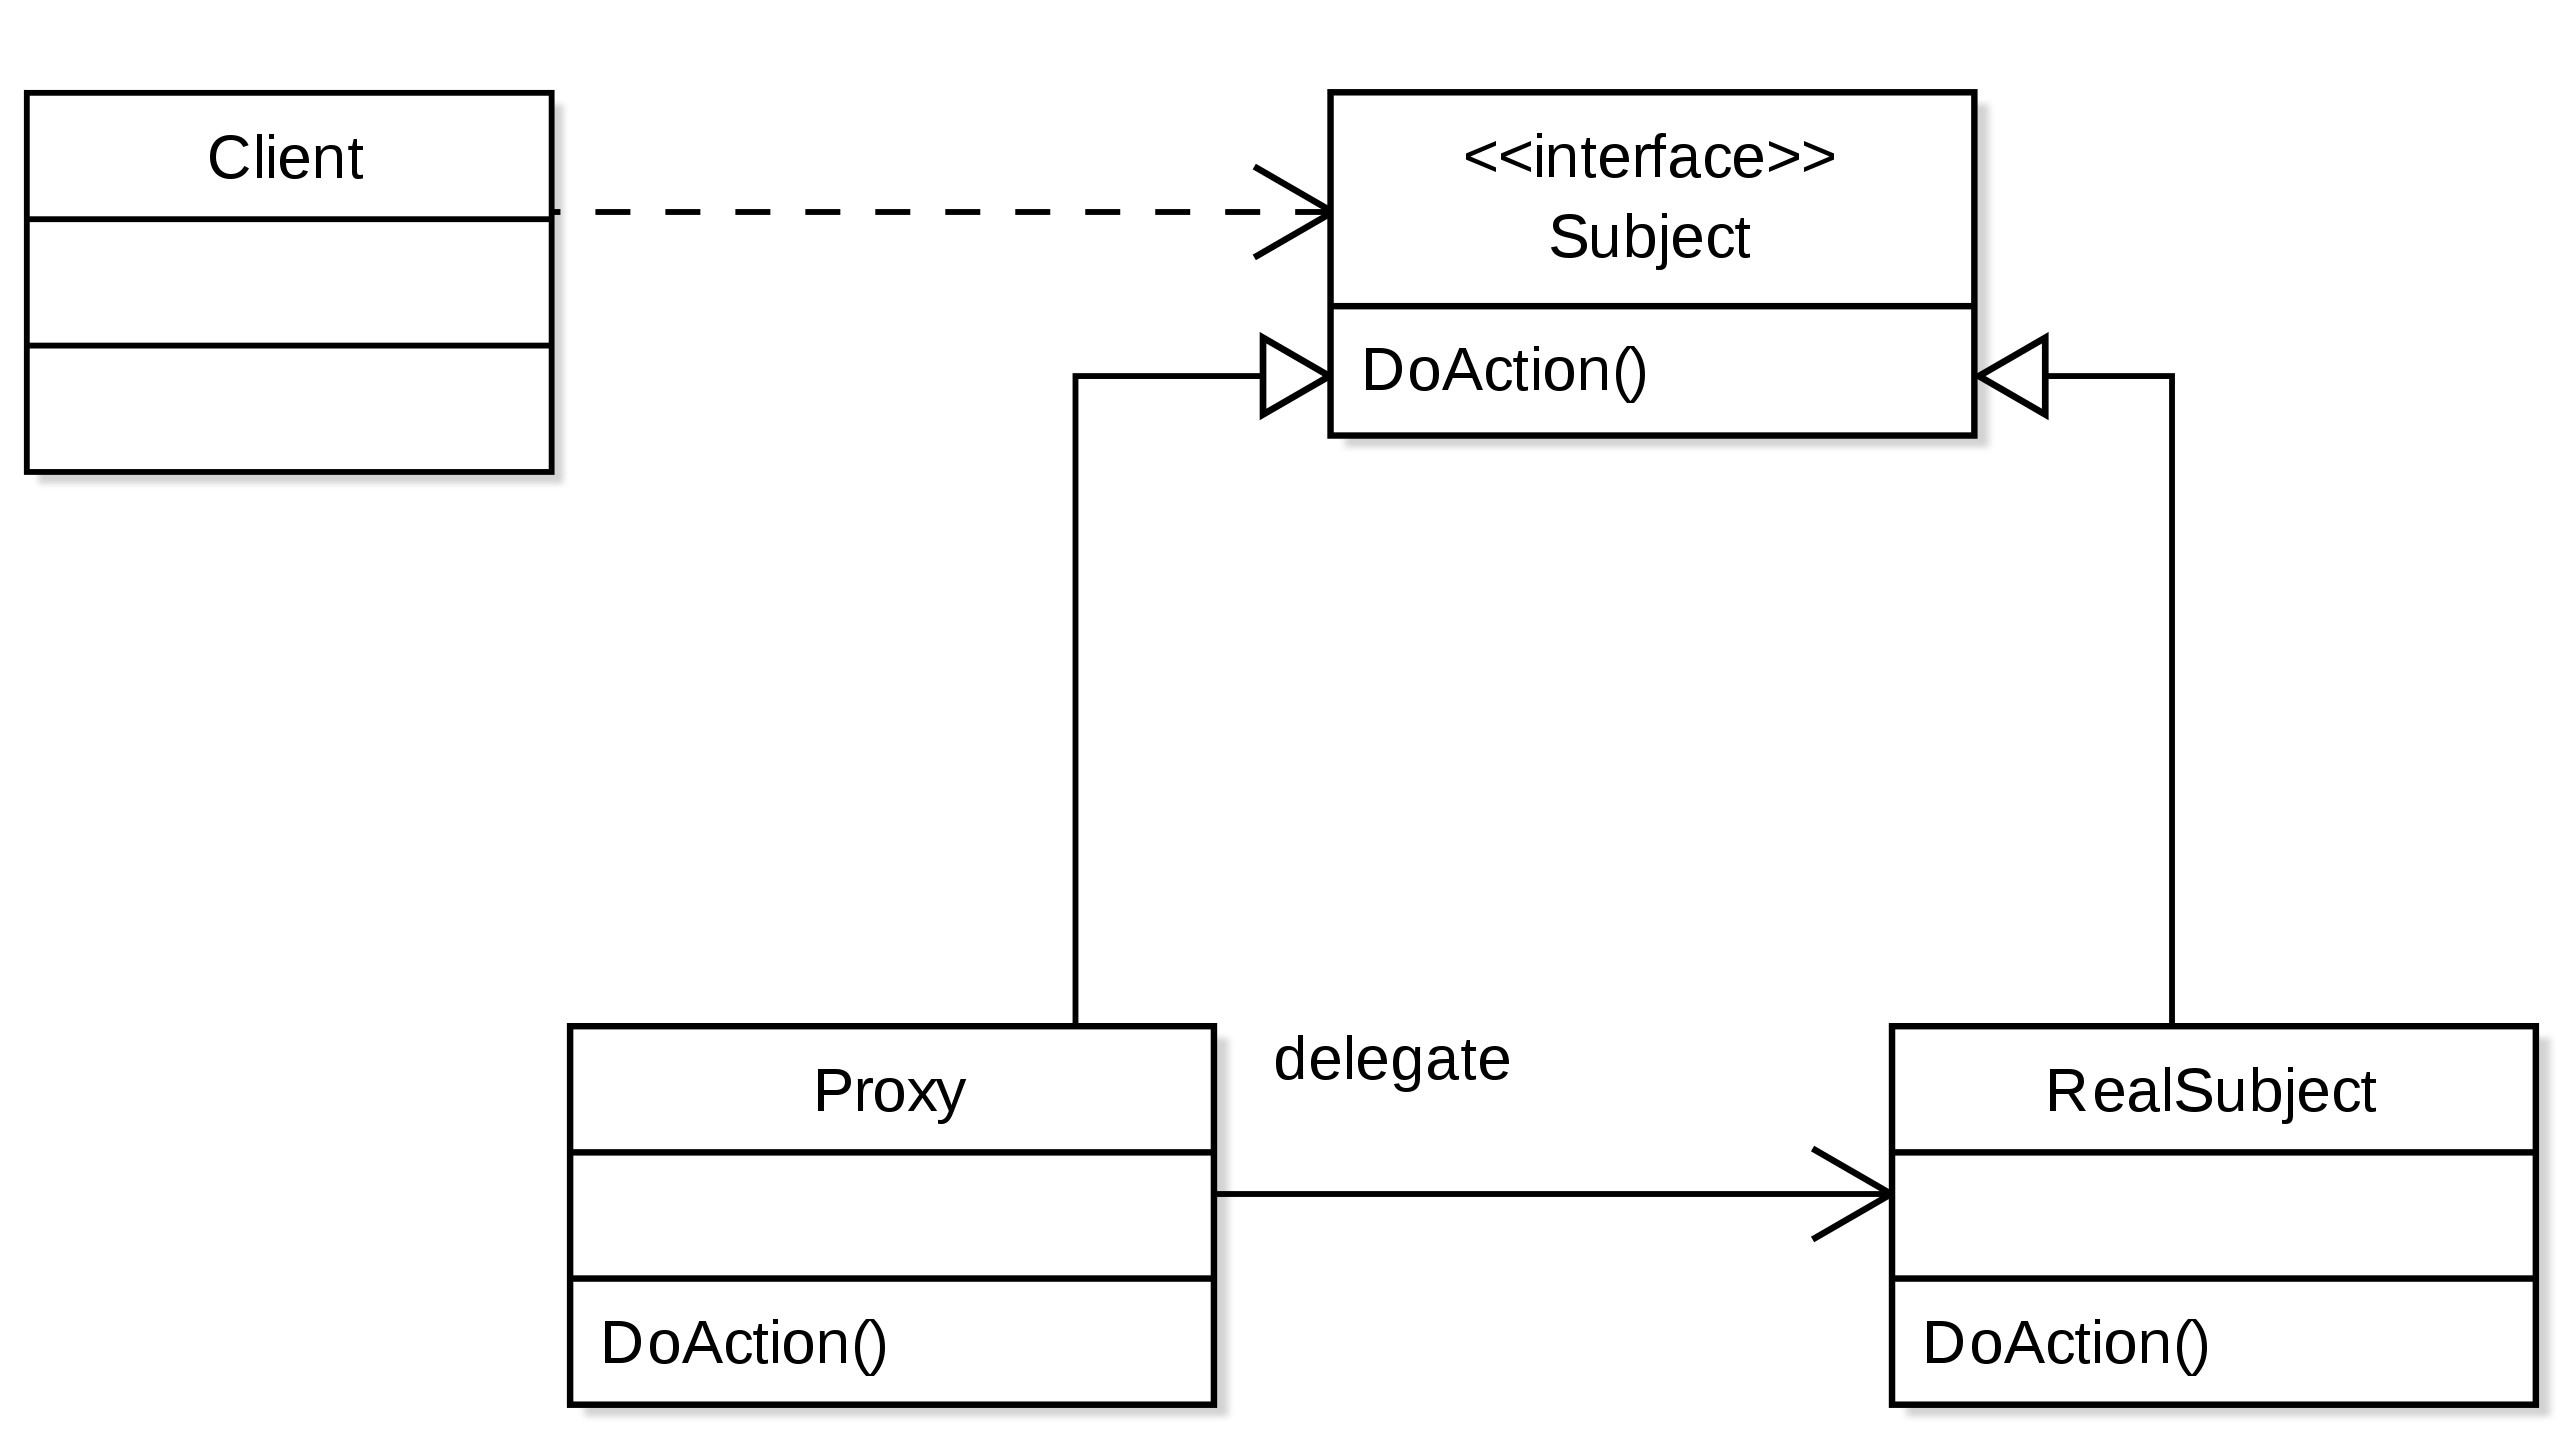
\includegraphics[width=1.0\linewidth]{../assets/images/2560px-Proxy_pattern_diagram.png}
	\end{figure}
\end{itemize}
\subsubsection{RAPS Architecture}
We want our system to rely on a RAPS (Reliable Array of Partitioned Service) architecture, in order to prevent unavailability of some functionalities in case of breakdowns. This architecture consists in a partitioned and redundant structure: servers are cloned to achieve this objective. More precisly, multiple services are divided on different machines and each machine can access in turn to a copy of the stored data. Such architecture guarantees better availability and scalability and provides a high rate of maintainability: in case of breakdowns, it is sufficient to work on the damaged machine, without interfering with the other machines' tasks, while the specific service can still be perfomed. In addition, if the system is willing to expand some services, it is sufficient invest
on the specific partition associated to that service.
\subsection{Other design decisions}

\section{USER INTERFACE DESIGN}
As already mentioned in the \texttt{Requirements Analysis and Specification Document} (RASD), our idea is to provide users with a Mobile App (for smartphones and tablets) and authorities with a Web App (for computers).\\ The applications will be different both in functionalities and in style, and we decided to separate the two and therefore make them exclusive, because of the different use and different authentication method they have.\\ For a closer look at what the two interfaces look like, we invite you to check our RASD where several mock-ups have been presented
\section{REQUIREMENTS TRACEABILITY}
\subsubsection*{[R1]: The system must allow users to provide their credentials and personal data}
\begin{itemize}
\item Components
\begin{itemize}
\item AuthenticationManager
\end{itemize}
\end{itemize}
\subsubsection*{[R2]: The system must let the user verify his account with his e-mail or by SMS}
\begin{itemize}
\item Components
\begin{itemize}
\item AuthenticationManager
\item SMS Service
\end{itemize}
\end{itemize}
\subsubsection*{[R3]: The system must verify there are no other registered users with the same e-mail or telephone number}
\begin{itemize}
\item Components
\begin{itemize}
\item AuthenticationManager
\item DBMS
\end{itemize}
\end{itemize}
\subsubsection*{[R4]: In order to register successfully, the system must oblige the user to accept the data privacy policies and conditions}
\begin{itemize}
\item Components
\begin{itemize}
\item AuthenticationManager
\end{itemize}
\end{itemize}
\subsubsection*{[R5]: The system must give the user the possibility to take pictures}
\begin{itemize}
\item Components
\begin{itemize}
\item Violations Report Module
\item Camera API
\end{itemize}
\end{itemize}
\subsubsection*{[R6]: The system must retrieve the users' position correctly}
\begin{itemize}
\item Components
\begin{itemize}
\item Main Thread Module
\item Maps API
\end{itemize}
\end{itemize}
\subsubsection*{[R7]: The system must recognize the license plate}
\begin{itemize}
\item Components
\begin{itemize}
\item ViolationsReportManager
\item OCR Module
\end{itemize}
\end{itemize}
\subsubsection*{[R8]: The system must give the user the chance to select a violation type from the dropdown menu}
\begin{itemize}
\item Components
\begin{itemize}
\item Violations Report Module
\end{itemize}
\end{itemize}
\subsubsection*{[R9]: The system musn't give the user the possibility to load photos from their device}
\begin{itemize}
\item Components
\begin{itemize}
\item Violations Report Module
\item Camera API
\end{itemize}
\end{itemize}
\subsubsection*{[R10]: If the users' wants to, the system must let them write an optional description.}
\begin{itemize}
\item Components
\begin{itemize}
\item Violations Report Module
\end{itemize}
\end{itemize}
\subsubsection*{[R11]: The system must show to the user all the violations he reported in the past}
\begin{itemize}
\item Components
\begin{itemize}
\item Profile Module
\end{itemize}
\end{itemize}
\subsubsection*{[R12]: The system must show to the user his account information and personal data when requested}
\begin{itemize}
\item Components
\begin{itemize}
\item Authentication Module
\end{itemize}
\end{itemize}
\subsubsection*{[R13]: The system must allow authorities to provide their credentials and personal authority identification}
\begin{itemize}
\item Components
\begin{itemize}
\item AuthenticationManager
\end{itemize}
\end{itemize}
\subsubsection*{[R14]: The system must verify there are no other registered authorities with the same identification}
\begin{itemize}
\item Components
\begin{itemize}
\item AuthenticationManager
\item DBMS
\end{itemize}
\end{itemize}
\subsubsection*{[R15]: In order to register successfully, the system must oblige the authority to accept the data privacy policies and conditions}
\begin{itemize}
\item Components
\begin{itemize}
\item AuthenticationManager
\end{itemize}
\end{itemize}
\subsubsection*{[R16]: The system must allow authorities to request a suggestion from SafeStreets}
\begin{itemize}
\item Components
\begin{itemize}
\item SuggestionManager
\item Municipality's Accidents Service
\item Machine Learning Module
\end{itemize}
\end{itemize}
\subsubsection*{[R17]: The system must allow authorities access to the Suggestions Map and see which suggestions have been posted for each area}
\begin{itemize}
\item Components
\begin{itemize}
\item Suggestion Module
\item Violations Retrieve Module
\item Maps API
\end{itemize}
\end{itemize}
\subsubsection*{[R18]: The system must allow authorities to discard pictures which don't represent a vehicle}
\begin{itemize}
\item Components
\begin{itemize}
\item Violations Retrieve Module
\item Pubblico Registro Automobilistico API 
\end{itemize}
\end{itemize}
\subsubsection*{[R19]: The system must allow authorities to discard pictures of vehicles which aren't committing any violation}
\begin{itemize}
\item Components
\begin{itemize}
\item Violations Retrieve Module
\item Pubblico Registro Automobilistico API 
\end{itemize}
\end{itemize}
\section{IMPLEMENTATION, INTEGRATION AND TEST PLAN}
\subsection{Implementation Plan}
We will implement our system one component/module at a time, according to a bottom-up approach that will facilitate a high deployment coverage in early phases. The order in which our implementation will be carried out, takes in account different factors such as the complexity of the modules and how they are interconnected with one another and we must take in consideration the possibility of discovering flaws and bugs in our designed system that will require to be fixed as soon as possible in order to prevent further additional costs and difficulties in debugging.\\\\
We can therefore implement our components in the order as follows:
\begin{itemize}
\item \textbf{Model}\\\\
This is the first component we are going to implement since all the parts of our Application Server will be using its elements and it allows services to communicate with the DBMS. It is therefore a crucial component for the entire system
\item \textbf{User Mobile Remote Services}\\\\
This is our first macro-component and it is made of the actual remote services that will interact with the modules of the user application. We will implement these services first as they will work as the foundations of our user-side application. We can see how all modules interact with the DBMS, the \texttt{Authentication Module} with the \texttt{SMS Service} and the \texttt{Violations Report Module} with the \texttt{OCR Module} (for recognizing the license plates)
\item \textbf{Authority Remote Services}\\\\
This is our second macro-component, as important as the \texttt{User Mobile Remote Services} as it works as a mirror to its functionalities, referring in fact to the authority side: here authorities exploit different functionalities but the most important is probably the \texttt{Suggestions Module} as it enables authorities to request suggestions on interventions to take on the streets, and it involves nearly all the parts of our system: the \texttt{Municipality's Accidents Service}, the \texttt{Machine Learning Module} and the DBMS.
\item \textbf{User Mobile Application}\\\\
Right after the two services, we will start implementing the actual applications: this is the one with which every user will be provided. While most of the components link to the actual services, some modules are linked to externals APIs such as the \texttt{Violations Report Module}, which needs to access the external \texttt{Camera API}, and the \texttt{Main Thread Module}, which needs to interact with the \texttt{Maps API}. 
\item \textbf{Authority Web Application}\\\\
Finally, we will implement the Web Application for authorities, having its foundations in the \texttt{Authority Remote Services}. Here authorities can interact with the above mentioned and its most important module, the \texttt{Violations Retrieve Module}, needs the \texttt{Pubblico Registro Automobilistico API} and the \texttt{Maps API} to work correctly
\end{itemize}
\subsection{Integration and Testing}
In the following sections we are going to illustrate how external components will be integrated with the ones implemented for the system and what testing strategy will be adopted.\\

This is the order in which we will integrate such components:
\begin{itemize}
\item \texttt{Integration with the DBMS}
\item \texttt{Integration with external services}
\item \texttt{Integration with the applications}
\end{itemize}
Every component will be integrated with various modules and/or external/internal services
\begin{itemize}
\item \textbf{Integration of the components with the DBMS}\\
Required integrations:
\begin{itemize}
\item \texttt{Authentication Module, DBMS}
\item \texttt{Profile Module, DBMS}
\item \texttt{Violations Report/Violations Retrieve Module, DBMS}
\item \texttt{Suggestions Module, DBMS}
\end{itemize}
\end{itemize}

\begin{itemize}
\item \textbf{Integration of the components with external services}\\
Required integrations:
\begin{itemize}
\item \texttt{Authentication Module, SMS Service}
\item \texttt{Violations Report Module, OCR Module}
\item \texttt{Violations Retrieve Module, Pubblico Registro Automobilistico API}
\item \texttt{Violations Retrieve Module, Maps API}
\item \texttt{Suggestions Module, Municipality's Accidents Service}
\item \texttt{Suggestions Module, Machine Learning Module}
\end{itemize}
\end{itemize}
\subsection{Components Integration}
In this section of the document,we will use some diagrams to describe how the components and subsystems of SafeStreets system will be linked to one another
\subsubsection{User Mobile Application Side Integration}
\begin{figure}[H]
		\centering
		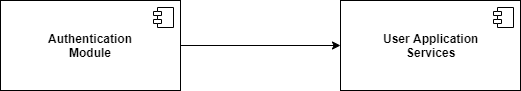
\includegraphics[width=0.5\linewidth]{../assets/images/auth_mod.png}
		\caption{Authentication Module links with the User Application Services}
\end{figure}
\begin{figure}[H]
		\centering
		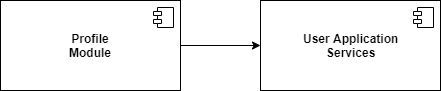
\includegraphics[width=0.5\linewidth]{../assets/images/prof_mod.png}
		\caption{Profile Module links with the User Application Services}
\end{figure}
\begin{figure}[H]
		\centering
		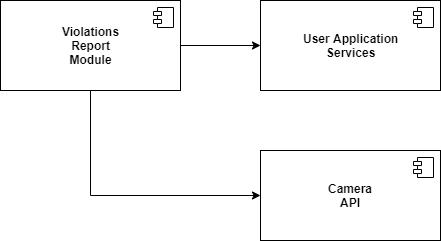
\includegraphics[width=0.5\linewidth]{../assets/images/viol_rep.png}
		\caption{This module is the users' most important and must have access to the Camera API}
\end{figure}
\begin{figure}[H]
		\centering
		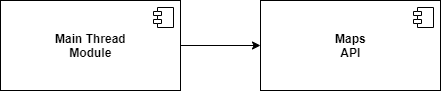
\includegraphics[width=0.5\linewidth]{../assets/images/main_thread_mod.png}
		\caption{This is the Main Thread Module and is composed only of the Maps API}
\end{figure}
\subsubsection{User Remote Services Side Integration}
\begin{figure}[H]
		\centering
		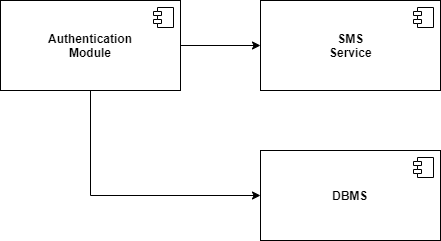
\includegraphics[width=0.5\linewidth]{../assets/images/auth_mod_serv.png}
		\caption{In the Remote Services, the Authentication Module interacts with the SMS Service and the DBMS}
\end{figure}
\begin{figure}[H]
		\centering
		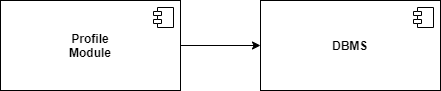
\includegraphics[width=0.5\linewidth]{../assets/images/prof_mod_serv.png}
		\caption{Profile Module links with the DBMS}
\end{figure}
\begin{figure}[H]
		\centering
		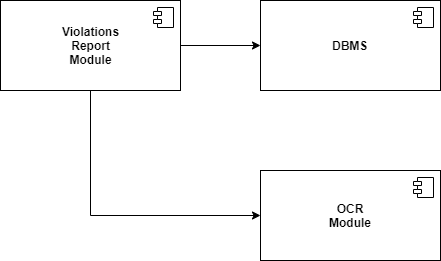
\includegraphics[width=0.5\linewidth]{../assets/images/viol_rep_serv.png}
		\caption{Once into the Remote Services, this module interacts with the OCR Module for plate recognition (together with the DBMS)}
\end{figure}
\subsubsection{Authority Web Application Side Integration}
\begin{figure}[H]
		\centering
		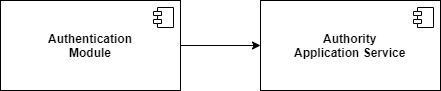
\includegraphics[width=0.5\linewidth]{../assets/images/auth_mod_auth.png}
		\caption{Authentication Module links with the Authority Application Services}
\end{figure}
\begin{figure}[H]
		\centering
		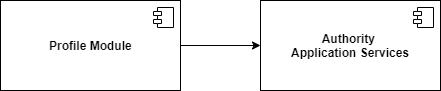
\includegraphics[width=0.5\linewidth]{../assets/images/prof_mod_auth.png}
		\caption{Profile Module links with the Authority Application Services}
\end{figure}
\begin{figure}[H]
		\centering
		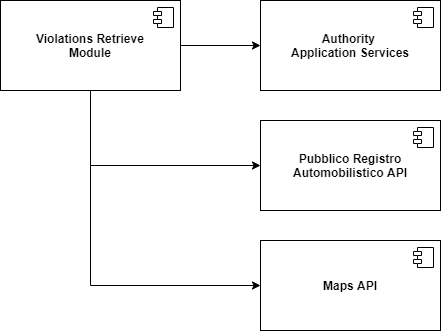
\includegraphics[width=0.5\linewidth]{../assets/images/viol_retr.png}
		\caption{This module is very important and links with the PRA API (in order to recognize the owner of the vehicle) and with the Maps API}
\end{figure}
\begin{figure}[H]
		\centering
		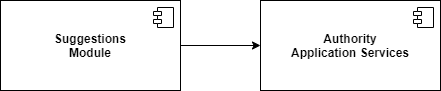
\includegraphics[width=0.5\linewidth]{../assets/images/sugg_mod.png}
		\caption{Suggestions Module links to Authority Application Services}
\end{figure}
\subsubsection{Authority Remote Services Side Integration}
\begin{figure}[H]
		\centering
		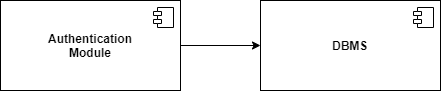
\includegraphics[width=0.5\linewidth]{../assets/images/auth_mod_auth_serv.png}
		\caption{Authentication Module links to the DBMS}
\end{figure}
\begin{figure}[H]
		\centering
		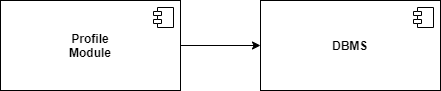
\includegraphics[width=0.5\linewidth]{../assets/images/prof_mod_auth_serv.png}
		\caption{Profile Module links to the DBMS}
\end{figure}
\begin{figure}[H]
		\centering
		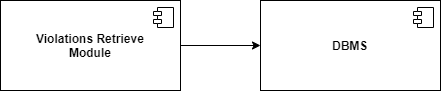
\includegraphics[width=0.5\linewidth]{../assets/images/viol_retr_serv.png}
		\caption{Violations Retrieve Module links to the DBMS}
\end{figure}
\begin{figure}[H]
		\centering
		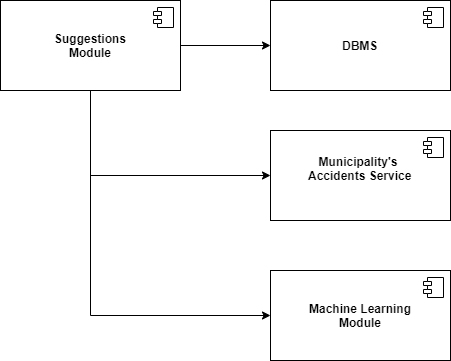
\includegraphics[width=0.5\linewidth]{../assets/images/sugg_mod_auth.png}
		\caption{This module is very important and links to the Municipality's Accidents Service (to retrieve information) and the Machine Learning Module (to generate suggestions)}
\end{figure}
\section{EFFORT SPENT}
\begin{itemize}
		\item Giancarlo Danese
		\begin{center}
			\begin{tabular}{| c | c | c |}
				\hline
				Day & Subject & Hours \\ \hline
				18/11/2019 & Purpose, Scope & 2 \\
				21/11/2019 & Architectural Design & 2\\
				24/11/2019 & Diagrams & 2\\
				27/11/2019 & Diagrams & 2\\
				30/11/2019 & Component View & 2\\
				03/12/2019 & Design Patterns & 2\\
				05/12/2019 & Requirements Traceability & 2\\
				08/12/2019 & Components Integration & 3\\
				09/12/2019 & UML & 3\\
				\hline
			\end{tabular}
		\end{center}

		\item Davide Savoldelli
		\begin{center}
			\begin{tabular}{| c | c | c |}
				\hline
				Day & Subject & Hours \\ \hline
				18/11/2019 & Architectural Design & 1 \\
				24/11/2019 & Diagrams & 2 \\
				27/11/2019 & Diagrams & 2 \\
				30/11/2019 & Deployment View & 2\\
				05/12/2019 & Requirements Traceability & 2\\
				08/12/2019 & Implementation Plan & 2\\
				09/12/2019 & Sequence Diagrams & 3\\
				\hline
			\end{tabular}
		\end{center}
	\end{itemize}
\section{REFERENCES}
\subsection{Reference Documents} 
\begin{itemize}
\item Specification Document "SafeStreets Mandatory Project Assignment"
\item "Appunti di Sistemi Informativi per il Settore dell'Informazione" A.Y 2017/2018
\item Wikipedia
\item Software Engineering 2 Course Slides
\end{itemize}
\subsection{Tools}
\begin{itemize}
\item \textbf{Draw.io}: https://www.draw.io/
\item \textbf{TeXWorks}: http://www.tug.org/texworks/
\item \textbf{Github Desktop}: https://github.com/
\end{itemize}
\end{document}
